Ein wichtiger schritt bei Erstellung eines Sentimentindizes ist die wahl des richtigen Wörterbuchs. Durch eine erste Visualisierung kann festgestellt werden, wie gut das ausgewählte Wörterbuch zur Fragestellung bzw. zum anfangs Problem passt.  Je nach dem welches Wörterbuch verwendet wird, für die Visualisierung von positiven und negativen Wörter, können sich die Ergebnisse verändern. Bei Betrachtung der Grafiken passen einigen Wörter sehr gut, wie fraud, stress, strike, win, support, top oder free und andere weniger gut, wie zum Beispiel fans, wow, die oder auch hate, zur Ausgangssituation einen Sentimentindex für Banken zubauen. In unseren Fall passt das ausgesuchte  Wörterbuch \textit{Bing} nicht optimal, aber insgesamt ganz gut.\\
\\
Mit mehreren Optionen für Sentiment Lexika's, ist es nötig mehr Informationen zu bekommen über diese Wörterbücher. Es werden alle vier Stimmungswörterbücher verwendet und untersucht, wie sich die Stimmung über die Wochen hinweg verändert. Zuerst benutzen wir die Funktion \textit{filter()}, um nur die Wörter aus dem einen Roman auszuwählen, der uns interessiert. Für die Wörterbücher \textit{Bing} und \textit{NRC} werden die positven und negativen Wörter pro Woche gezählt und miteinander verrechnet um einen Sentimenindex zu bilden. Die Wörterbücher \textit{NRC} und \textit{Warp} besitzen einen Score für jedes Wort schon.
\begin{figure}[H]
	\centering
	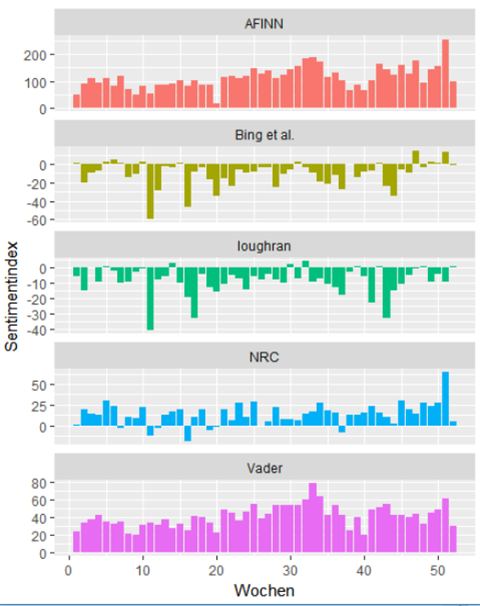
\includegraphics[width=1\textwidth]{C:/Users/Christian/Documents/textmining/R-projekt/BeckerSeminar2/Reporting/Woertbuch.png}
	\caption{Sentimentindiezes Wörterbücher}
	\label{senti}
\end{figure}
Es sind ähnliche Einbrüche und Stimmungsspitzen an ungefähr den gleichen Stellen bei den Tweets zuerkennen, aber die absoluten Werte sind signifikant unterschiedlich. Das \textit{AFINN}$\-$ und \textit{Wap} Wörterbuch geben die größten absoluten Werte an, mit hohen positiven Werten. Das Lexikon von \textit{Bing} hat niedrigere Absolutwerte und scheint größere Blöcke zusammenhängenden positiven oder negativen Textes zu bezeichnen. Die \textit{NRC} und \textit{Warp}$\-$Ergebnisse sind im Vergleich zu den beiden anderen in der Höhe verschoben, wodurch der Text positivere Werte verzeichnet, aber ähnliche relative Veränderungen im Text erkannt werden. Wir finden ähnliche Unterschiede zwischen den Methoden, wenn wir uns andere Tweets anschauen; das \textit{NRC}$\-$Sentiment ist hoch, das \textit{AFINN}$\-$Sentiment hat mehr Varianz, \textit{Warp} hat ein ähnliches Verhalten, wie das \textit{NRC}$\-$Sentiment, das \textit{Bing} sentiment scheint Wochen die nahe bei einander liegen ähnlichen zu zu bewerten, aber alle vier sind sich über die allgemeinen Tendenzen des Sentimentes einig.

Warum weißt z.B. das Ergebnis für das \textit{NRC}$\-$Lexikon im Vergleich zum \textit{Bing et al.} positvere Stimmung?  Hierzu wird geprüft, wie viele positive und negative Wörter in diesen Wörterbücher enthalten sind.
Das Wörterbuch \textit{NRC} besitzt $3324$ negative und $2312$ positive Wörter. Im Gegensatz beträgt das Lexika \textit{Bing} $4782$ negative und $2006$ positive Wörter, damit besitzt die Wörterliste \textit{Bing} eine größere Anzahl von positiven Wörter. 
\subsection{Übereinstimmungen von Sentimentindizes mit Aktienkurse}
In diesem Abschnitt wird ein kurzes Resume gezogen, in wie weit der Sentimentsindex der Bankentweets aus $2012$ in der USA und der EU mit der wirtschaftlichen Situation in $2012$ übereinstimmt. Für den Vergleich der wirtschaftlichen Situation in der EU, wird der \textit{EURO-STOXX} $50$ herangezogen. Der \textit{EURO-STOXX} $50$ ist ein Aktienindex, der sich aus $50$ großen, börsennotierten Unternehmen des Euro-Währungsgebiets zusammensetzt. Er gilt als eines der führenden Börsenbarometer Europas und enthält die Aktien von $50$ Unternehmen aus Euroländern. Der Dow Jones wird für die US-Banken-Tweets genommen.

Um ein Bild der Stimmung in den Tweets zu erhalten, sollen die Anzahl der positiven und negativen Wörter pro Monat gezählt werden und die Differenz genommen werden, dazu wird das Wörterbuch \textit{Bing} verwendet.
\begin{figure}[H]
	\begin{minipage}[b]{.4\linewidth} % [b] => Ausrichtung an \caption
		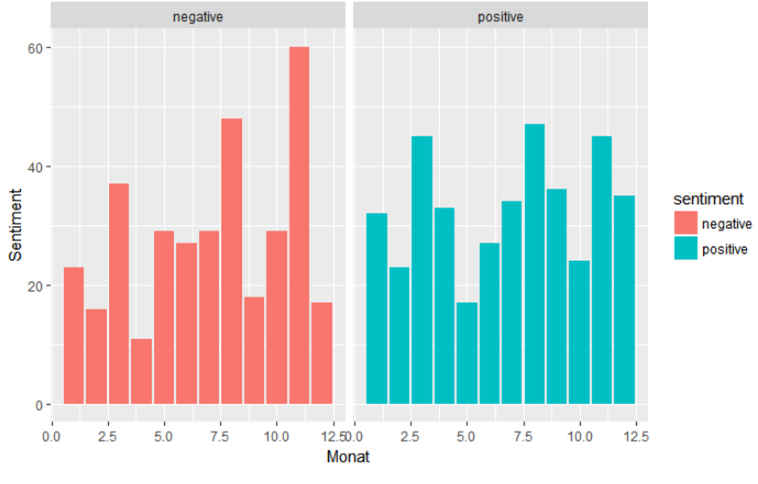
\includegraphics[width=1\textwidth]{C:/Users/Christian/Documents/textmining/R-projekt/BeckerSeminar2/Reporting/EUpostneg.png}
		\caption{Sentimentindex EU-Banken positve und negative Wörter pro Monat} \label{eusent}
	\end{minipage}
	\hspace{.1\linewidth}% Abstand zwischen Bilder
	\begin{minipage}[b]{.4\linewidth} % [b] => Ausrichtung an \caption
		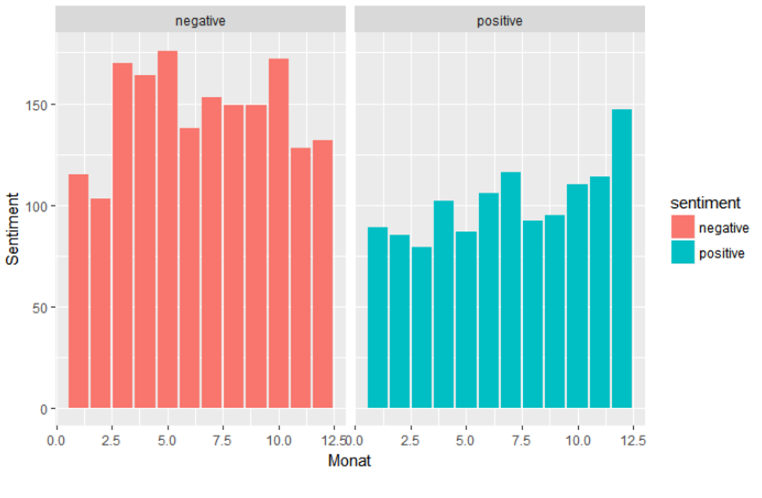
\includegraphics[width=1\textwidth]{C:/Users/Christian/Documents/textmining/R-projekt/BeckerSeminar2/Reporting/USApostneg.png}
		\caption{Sentimentindex USA-Bankenbpositve und negative Wörter pro Monat}\label{usasent}
	\end{minipage}

	\begin{minipage}[b]{.4\linewidth} % [b] => Ausrichtung an \caption
	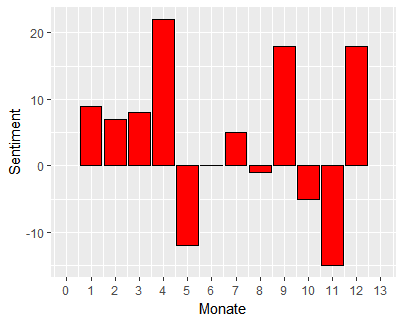
\includegraphics[width=1\textwidth]{C:/Users/Christian/Documents/textmining/R-projekt/BeckerSeminar2/Reporting/Monateu.png}
	\caption{Sentimentindex EU-Banken differenz  zwischen positve und negative Wörter pro Monat}\label{eudiff}
\end{minipage}
	\hspace{.2\linewidth}
\begin{minipage}[b]{.4\linewidth} % [b] => Ausrichtung an \caption
	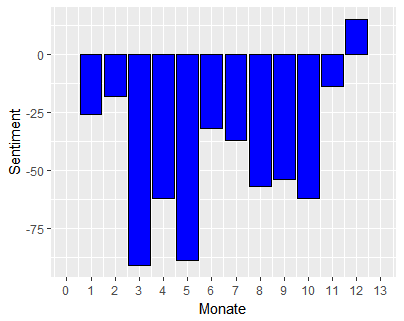
\includegraphics[width=1\textwidth]{C:/Users/Christian/Documents/textmining/R-projekt/BeckerSeminar2/Reporting/Monatusa.png}
	\caption{Sentimentindex USA-Banken differenz  zwischen positve und negativen Wörter pro Monat}\label{usadiff}
\end{minipage}
\end{figure}
In den Grafiken \ref{usasent} und \ref{usadiff} der Tweets der US-Banken  ist abzulesen, dass es mehr negative als positive Wörter gibt, in den Monaten Januar bis November. Die Sentiments in den Plots \ref{eusent} und \ref{eudiff} der Tweets der EU-Banken sind sehr wechselhaft. Die Monaten Mai, Juni, August, Oktober und November besitzen mehr negative als positive Wörter. Es werden die Hoch und tiefst der obigen Grafiken mit dem Aktienkurs des \textit{Dow Jones} und \textit{Euro Stoxx} $50$ aus $2012$ auf Gemeinsamkeiten untersucht. 
 \begin{figure}[H]
 \begin{minipage}[b]{.4\linewidth} % [b] => Ausrichtung an \caption
 	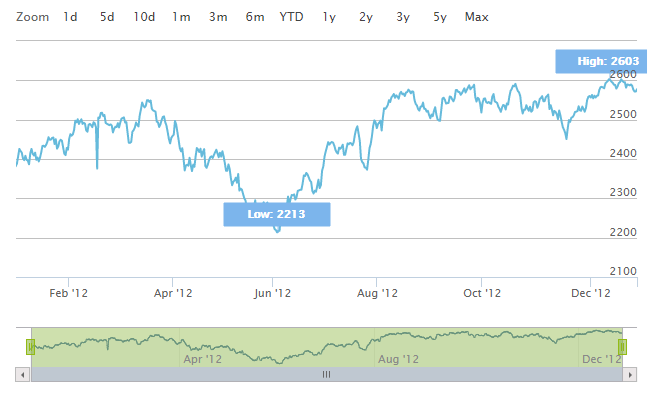
\includegraphics[width=1\textwidth]{C:/Users/Christian/Documents/textmining/R-projekt/BeckerSeminar2/Reporting/EuroxStoxx.png}
 	\caption{Euro Stoxx $50$ Aktienkurs $2012$} \label{eustoxx}
 \end{minipage}
 \hspace{.1\linewidth}% Abstand zwischen Bilder
 \begin{minipage}[b]{.4\linewidth} % [b] => Ausrichtung an \caption
 	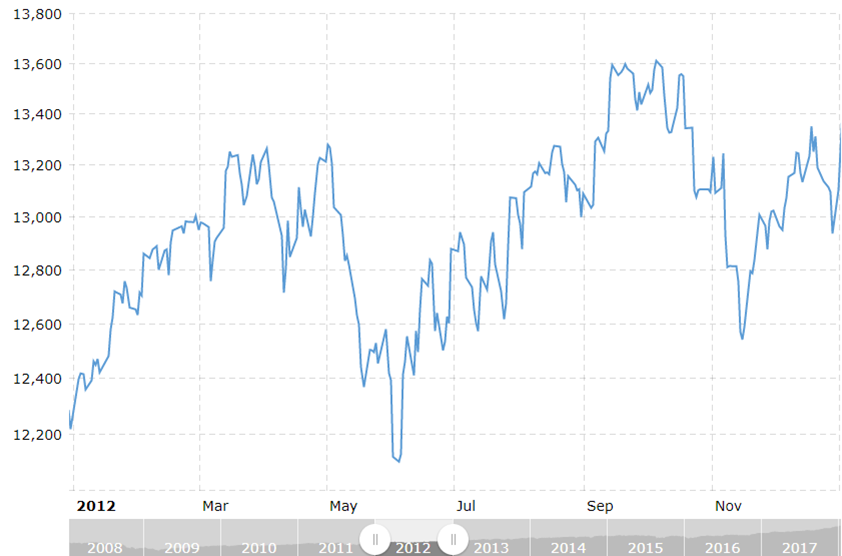
\includegraphics[width=1\textwidth]{C:/Users/Christian/Documents/textmining/R-projekt/BeckerSeminar2/Reporting/DowJones2012.png}
 	\caption{Dow Jones Aktienkurs $2012$}\label{dowjones}
 \end{minipage}
\end{figure}
Der \textit{Euro Stoxx} $50$ Aktienkurs Chart $2012$ zeigt in den Monaten Mai und Juni einen Kurssturz an und im August erholt, diese Information passt auch mit dem Sentiments in den Tweets überein. In der Phase des Aktiensturz  die Mai liegt gibt es einen starken anstieg an negativen Tweets. Im Juni ist der Tief stand erreicht und der Aktienkurs steigt wieder an, die Anzahl der negative Wörter ist leicht zurückgegangen und die Anzahl der positiven Wörter angestiegen. Im August ist zu ein Aktieneinbruch zu erkennen, dieser wirkt sich negative auf den Sentiment im August aus. Es existieren gering mehr negative als positive Wörter im Monat August. Dies lässt die Annahme aufkommen, dass dieser kurze Aktieneinsturz im August ein erhebliche Reaktion an negativen Tweets auslöste. In der Grafik \ref{eustoxx} zeichnet sich Weiterhin im September eine Trendphase ungefähr bis Oktober ab. Dieser Trend scheint auch in den Tweets sichtbar zu werden, da es mehr positive als negative Wörter im Monat September vorhanden sind. Auch der Aktienkurs vom Dow Jones (\ref{dowjones}) und der Sentimentindex der Tweets der US-Banken (\ref{usadiff}) aus $2012$. Im März und im April steigen die Anzahl von negativen Wörter stark an, wie in der Grafik \ref{usadiff} zuerkennen ist und nehmen nach Mai verstärkt wieder ab. Dieser Effekt stimmt mit dem Verhalten des Aktienkurs des Dow Jones überein. Im März und Mai gibt es einen Einbruch und anschließend einen Trend. Es kann festgehalten werden, dass das Zählen von positiven und negativen Wörter pro Monat, die Stimmung in der Finanzwelt grob erfassen kann. Im nächsten Abschnitt wird mittels verschiedener Sentimentindizes von mehreren Wochen eine multiple Regression auf wöchentliche Renditen.
\section{Modell} 

Dieses Kaptiel setzt statistische Grundlagen voraus, die im Bachelor der Angewandte Mathematik in \textit{Statistik 1} und \textit{Statistik 2} behandelt wurden. 
Im Rahmen der empirischen Untersuchung wird die klassische multiple Regression verwendet. Ziel der multiplen Regression auf wöchentliche Renditen von Aktienkursen ist es, die Kursentwicklung einer Aktie durch die Entwicklung eines zugehörigen Sentimentindexes zu erklären und vorherzusagen. Mithilfe historischer Zeitreihen/Kursen wird versucht den Zusammenhang zwischen der Rendite eines einzelnen Wertpapiers und einem Sentimentindex zu ermitteln, um mit Hilfe des gewonnenen Zusammenhangs zukünftige Renditen des Wertpapiers zu schätzen. \\

Die künftigen Renditen der Aktienkurse werden ausschließlich
durch den linearen Zusammenhang zu den Sentimentindizes der letzten Wochen geschätzt. Mit Hilfe einer multiplen linearen Einfachregression wird eine Schätzung für zukünftige Renditen des Aktienkurses erstellt, da ein linearer Zusammenhang zwischen der Rendite des einzelnen Wertpapiers und der Sentimentindizes vorausgesetzt wird. Einen gewissen Zusammenhang wurde zwischen einem einfachen Sentimentindex, der positive und negative Wörter zählt und als Score die Differenz nimmt, und der Rendite des Aktienkurses  Dow Jones aufgezeigt, im  vorherigen Abschnitt beschrieben. Es ergibt sich folgende lineare Regressionsgleichung:
\begin{equation}
r_{t}=\alpha_{t}+ \sum_{k=1}^{K} \beta_{k} S_{k}+\varepsilon_{t}
\end{equation}
mit:
\begin{itemize}
	\item  $R_{t}$ sind die wöchentlichen Renditen bzw. prozentuale Veränderung des Aktienkurses
	\item $S_{k}$ ist der Sentimentindex der letzten $k$ Wochen und $\beta_{k}$ ist der dazugehörige Betakoeffizent
	\item $\varepsilon_{t}$ für  Fehlerterm 
\end{itemize}
Im Folgendem wird nun versucht mit verschiedene Sentimentindizes auf den \textit{Dow Jones Industrial} $30$ Renditen vorherzusagen. Zu Beginn verwenden wir als Sentimentindex für die multiple Regression, die Differenz der Anzahl von positive und negative Wörter pro Woche der US-Banken-Tweets. Der Dataframe mit den Indizes muss nun mit dem Dataframe der Renditen  des \textit{Dow Jones Inustrial} $30$ gejoint werden, über das Feld \textit{week}. Für die Modellierung der Regressionsgleichung ist es erforderlich, sich zu überlegen, inwieweit der linearen Zusammenhang der Rendite zu den Sentimentindizes der letzten Wochen sinnvoll ist. \\
\\
\textbf{Wie viel Wochen der Vergangenheit von Zeitpunkt heute muss mitgenommen werden, damit keine wichtigen Informationen verloren gehen?} 
\\
\\
Dies kann nur empirisch ermittelt werden. In unserem Fall gehen wir von der Hypothese aus, dass drei bis vier Wochen ein erster vernünftiger Startpunkt ist. Im nächsten Schritt wird eine Regression mit den Sentimentindizes der letzten drei Wochen durchgeführt werden. Hierzu muss mit der Funktion \textit{generateLinearRegressionDataFrame} unsere Dataframe in die richtige Form transformiert werden. In der unteren R Ausgabe sind die Ergebnisse Regression zu sehen. Auf den ersten Blick fällt auf, dass nach dem T-Test alle $H_{0}$ Hypothesen für die Regressionskoeffizienten nicht verworfen werden können, da alle $\alpha>0.05$ sind, wie in der Tabelle \textit{Coefficients} in der Spalte $Pr(>|t|)$ zu sehen ist. Daraus folgt die Sentimentinidizes der letzen drei Wochen besitzen keinen Einfluss auf die Renditen (wöchentliche Veränderung pro Woche)  des \textit{Dow Jones Industrial} $30$. Diese Ergebnisse sind nicht ungewöhnlich, da wir nicht mehr in der normalen multiplen Regression uns bewegen, sondern im Bereich der Zeitreihenanalyse schon, da zeitliche Ereignisse betrachtet werden.
 \begin{figure}[H]
   	\centering
  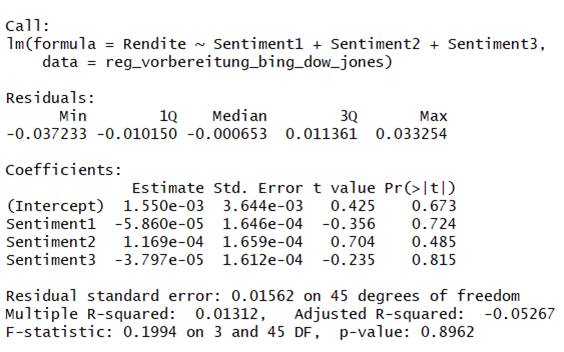
\includegraphics[width=1\textwidth]{Pictures/ergebnisse_sentiment.png}
   	\caption{Summary der multiplen Regression}
\end{figure}
 \begin{figure}[H]
	\centering
	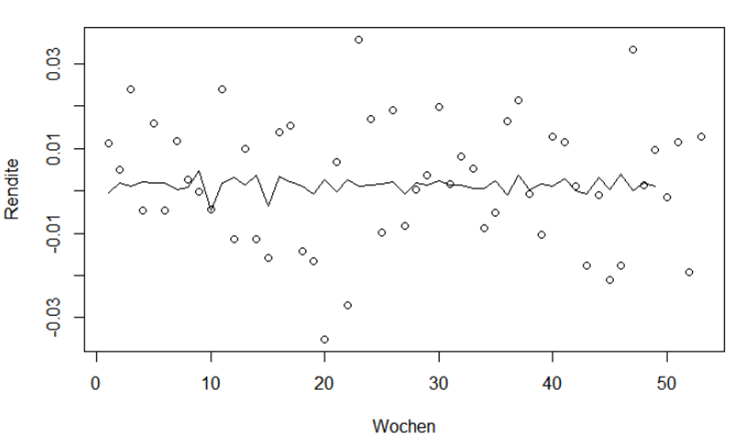
\includegraphics[width=1\textwidth]{Pictures/Regression_bing_diff.png}
	\caption{Plot der Regression}
\end{figure}


url https://www.stoxx.com/index-details?symbol=SX5P
https://www.boerse.de/boersenlexikon/EURO-STOXX
